\Chapter{Hasonló célú szoftverek és szolgáltatások}

Ebben a fejezetben arról lesz szó, hogy milyen fajta használtautó hirdető és milyen aggregáló web alkalmazások léteznek. Betekintést szerzünk arról, hogy milyen hasonló szoftverek léteznek, ahhoz amilyenről később majd bővebb szót fogok ejteni.

\Section{Használtautó hirdető oldalak.}

Mióta elkezdték gyártani a különböző gépjárműveket, azóta van lehetőségük az embe-
reknek használtautók megvásárlására. Eleinte csak a heti lapok hirdetés rovatában látták, ha valaki árulta az autóját és ott csak leírást láttak az autóról nem volt kép. Ahogyan telt az idő jelentek meg különböző autós témájú újságok, ahol lehetett autókat hirdetni méghozzá már képpel, így már vizuálisan is látható volt az autó. 
Mikor bejött az internet és egyre jobban elterjedt az emberek között, akkor elkezdtek fejleszteni különböző web alkalmazásokat volt közöttük olyan is, amit használtautó hirdetésre fejlesztettek ki. Számtalan ilyen oldal található meg, de van kettő, ami nekem személyes kedvencem az egyik a JóAutók.hu[link] a másik pedig a Használtautó.hu[link].

\subsection{JóAutók}
A JóAutók csak autók hirdetésére alkalmas más gépjárművek vagy motorkerékpárok nem találhatóak meg rajta. Van az oldalon lehetőség autók keresésére és hirdetés feladására is, de a hirdetéshez először regisztrálni kell.

Ha böngészni szeretnénk az autók között, akkor először ki kell választani az autót keresek menüpontot ami után megjelenik egy új oldal és már el is kezdhetjük a keresést.

Ha nekünk nem tetszik az, hogy az összes autót kiadja, az oldal akkor van lehetőség szűrni különböző feltételek szerint, mint például:
\begin{itemize}
\item márka
\item ha szűrünk márkára, akkor modell
\item megyére is lehet, hogy milyen megyében keresünk autót
\item kivitel
\item árára
\end{itemize}

és még rengeteg szűrési lehetőség van, bárki meg tudja rajta keresni a neki megfelelő autót.

\begin{figure}[h]
\centering
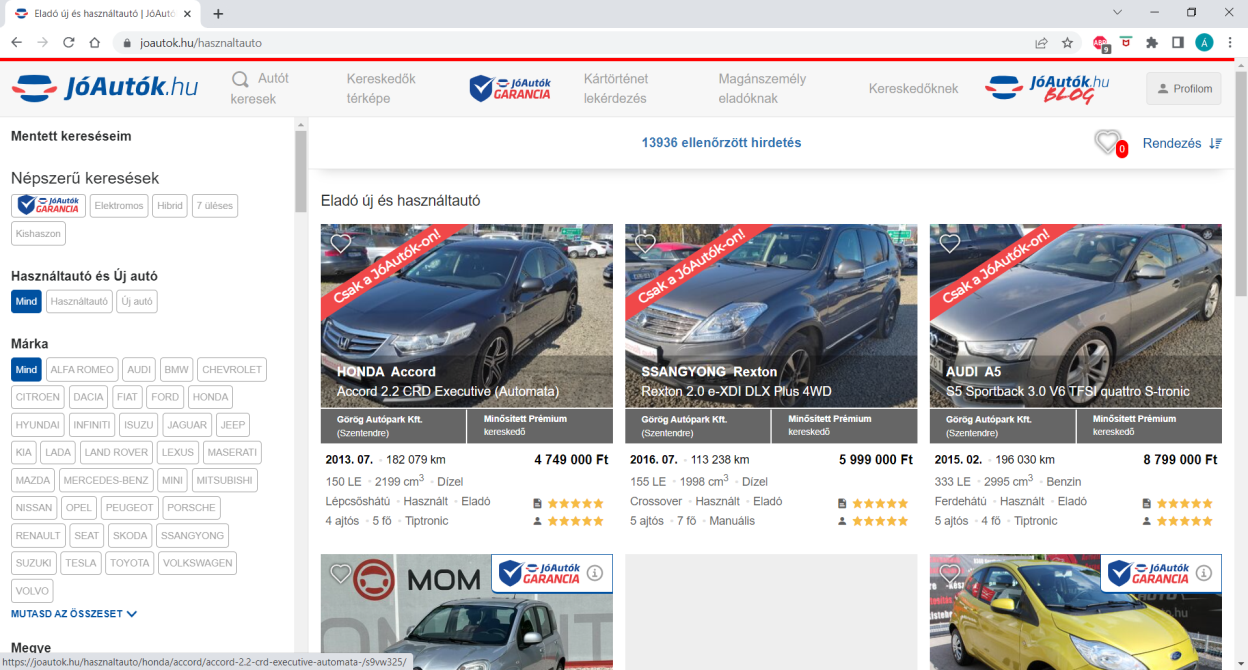
\includegraphics[scale=1]{images/joautok.png}
\caption{joautok.hu\cite{JoAuto}}
\label{fig:joautok}
\end{figure}

\subsection{Használtautó.hu}

Használtautó.hu szerintem Magyarország legnépszerűbb használtjármű oldala. Ezen a weboldalon személyautótól kezdve munkagépeken keresztül hajók, autóbuszok és lakókocsik vásárlására és eladására is van lehetőség, tehát egy nagyon széles körű weboldalról beszélünk.

A JóAutóktól eltérően itt először meg tudjuk adni a keresési feltételeinket, hogy milyen autók hirdetéseit szeretnénk látni.

\begin{figure}[h]
\centering
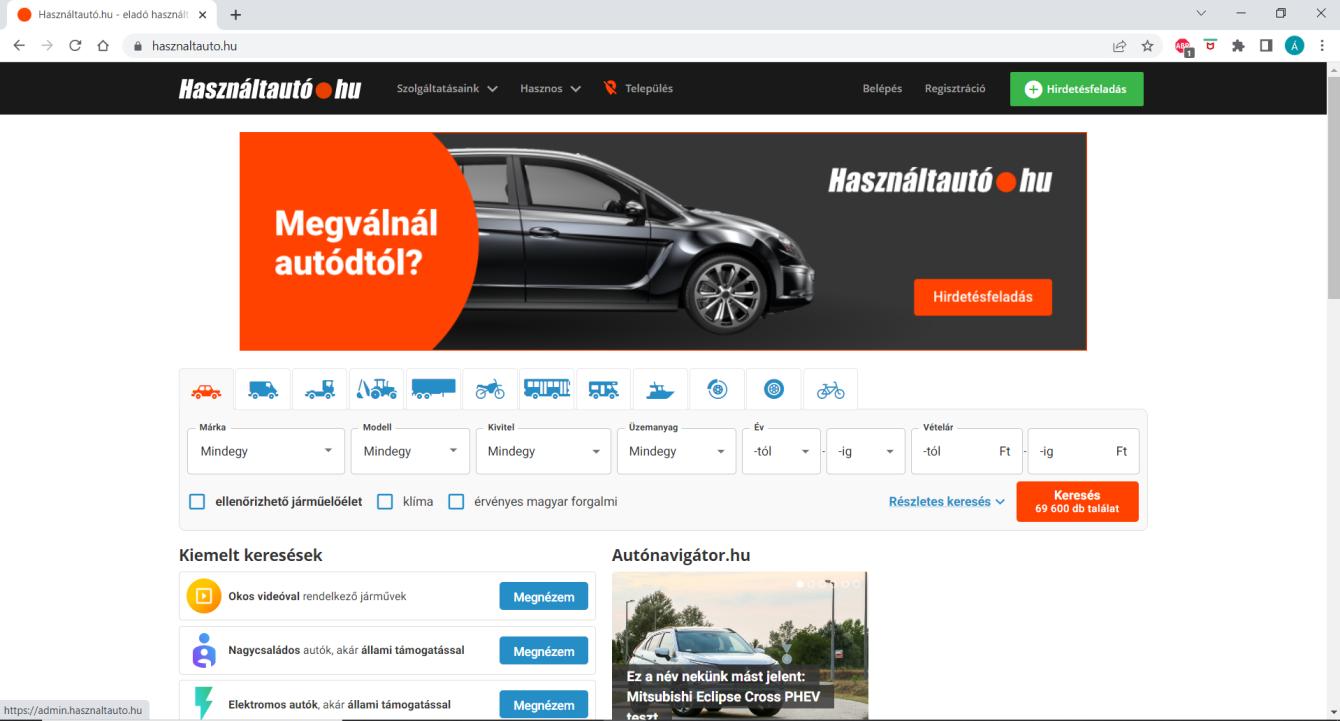
\includegraphics[scale=0.8]{images/hasznaltauto.png}
\caption{hasznaltauto.hu\cite{Hasznaltauto}}
\label{fig:hasznaltauto}
\end{figure}
\newpage

Használtautónak van egy olyan jó funkciója, amit úgy hívnak, hogy „Okos videó” ami azt jelenti, hogy egy rövid kis videóban végig mutatja az autóról feltöltött képeket és közben megjelennek az autó paraméterei is hogy mennyi kilométer van benne, milyen évjáratú, milyen üzemanyagot fogyaszt. 

\Section{Aggregáló oldalak}

Az aggregáló oldalaknak az a lényege, hogy több oldalról gyűjti össze az információkat egy témáról, árukról vagy éppen össze gyűjti egy adott termékről az összes elérhető boltot ahol árulják őket és a vásárlónak lehetősége van itt össze hasonlítani az árakat és kitudja választani a számára legmegfelelőbb boltot.

\subsection{Árukereső}

Az árukereső pont egy olyan weboldal, ahol az ember szétnézhet, össze tudja rajta hasonlítani az árakat és a termékek közötti különbségeket, hogy kiválassza az adott ár kategóriában a legjobb terméket.

Rengetek kategória érhető el az oldalon, tehát szinte bármi megtalálható rajta amit csak szeretne venni egy átlagember mint például:

\begin{itemize}
\item Ajándékok
\item Hobbi felszerelések
\item játékok
\item Műszaki cikkek
\end{itemize}

Ezt az alábbi kép is szemlélteti:

\begin{figure}[h]
\centering
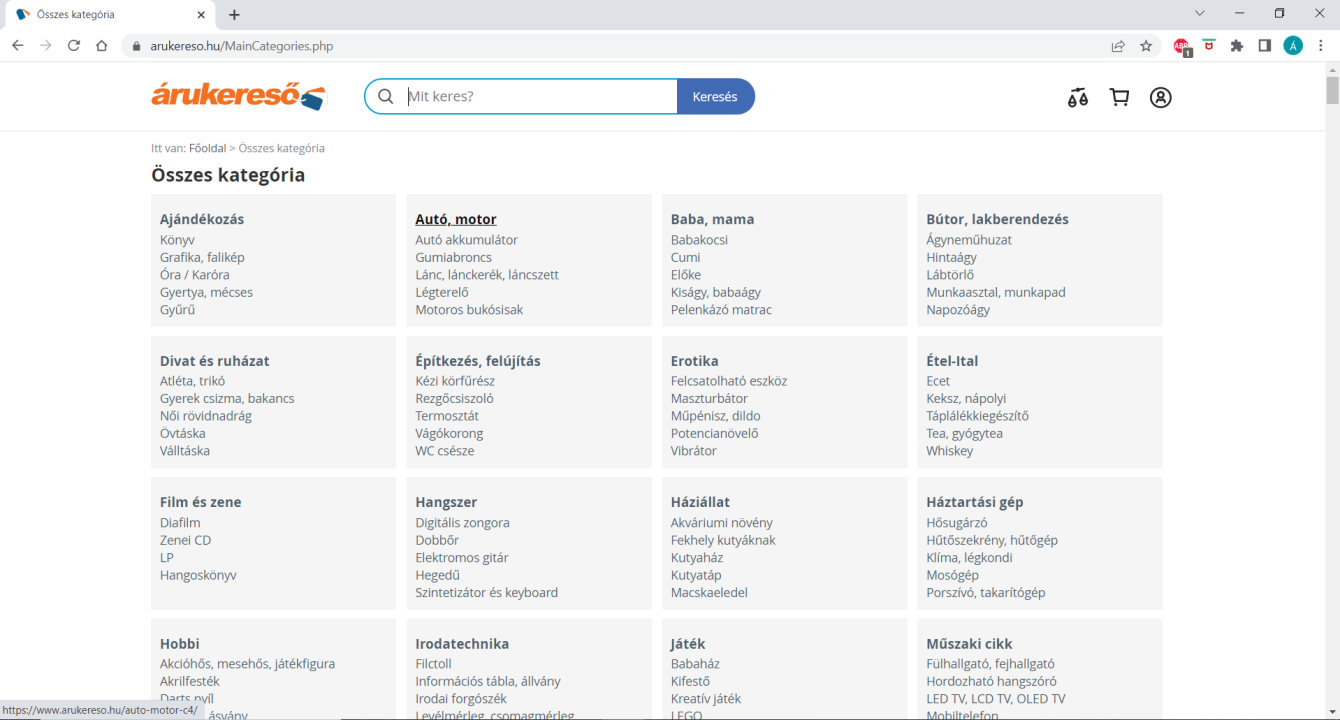
\includegraphics[scale=0.8]{images/arukereso.png}
\caption{Az árukereső kategória választója\cite{Arukereso}}
\label{fig:arukereso}
\end{figure}
\newpage